\subsubsection{Data Augmentation}
Data augmentation is a technique to artificially create new training data from existing training data. This is done by applying domain-specific techniques to examples from the training data that create new and different training examples.\newline
Image data augmentation is perhaps the most well-known type of data augmentation and involves creating transformed versions of images in the training dataset that belong to the same class as the original image.\newline
Transforms include a range of operations from the field of image manipulation, such as shifts, flips, zooms, and much more, also we need to choose it carefully and not apply any type of operation that do not match the actual situations our model face.(see Figure~\ref{fig:data_augmentation})
\begin{figure}
	\centering
	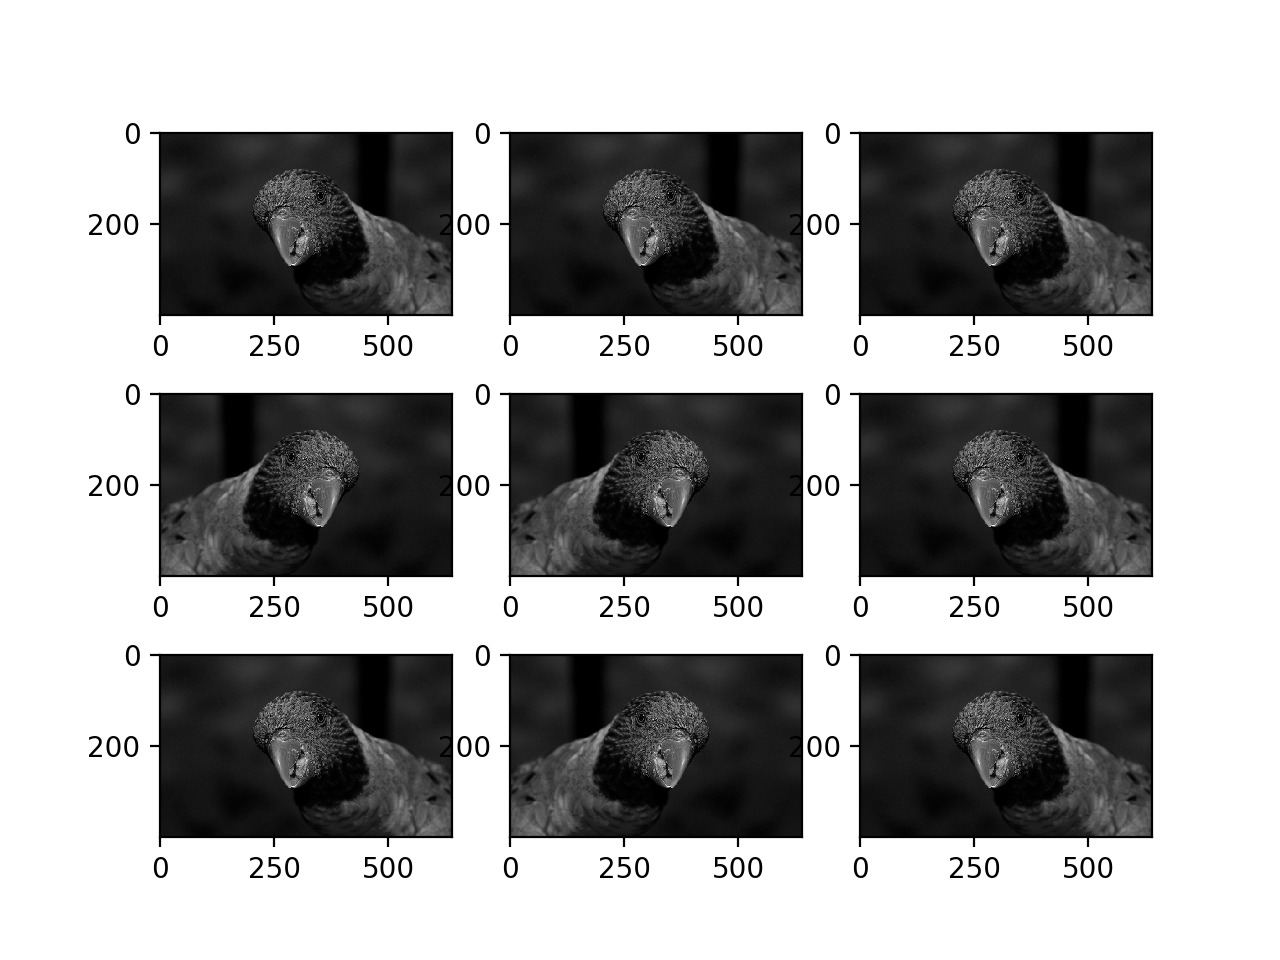
\includegraphics[width=1\textwidth]{images/data_aug.jpg}
	\caption{example of Data Augmentation "Horizontal flip"}
	\label{fig:data_augmentation}
\end{figure} 
\newline
Image data augmentation is typically only applied to the training dataset, and not to the validation or test dataset. This is different from data preparation which must be performed consistently across all dataset images.




